%
% Tutorial -- Getting Started with Qucs
%
% Copyright (C) 2007 Stefan Jahn <stefan@lkcc.org>
% Copyright (C) 2007 Juan Carlos Borr�s <jcborras@gmail.com>
%
% Permission is granted to copy, distribute and/or modify this document
% under the terms of the GNU Free Documentation License, Version 1.1
% or any later version published by the Free Software Foundation.
%

\tutsection{Introduction}

The following sections are meant to give an overview about what the
Qucs software can be used for and how it is used to achieve this.

\medskip

Qucs is free software licensed under the General Public License (GPL).
It can be downloaded from \url{http://qucs.sourceforge.net} and comes
with the complete source code.  Every user of the program is allowed
and called upon (on a voluntary basis of course) to modify it for
their purposes as long as changes are made public.  Contact the
authors to verify them and finally to incorporate it into the
software.

\medskip

The software is available for a variety of operating systems including
\begin{itemize}
\item GNU/Linux
\item Windows
\item FreeBSD
\item MacOS
\item NetBSD
\item Solaris
\end{itemize}

On the homepage you'll find the source code to build and install the
software.  Build instructions are given.  Also links for binary
packages for certain distributions (e.g. Debian, SuSE, Fedora) can be
found.

\medskip

Once the software has been successfully installed on your system you
can start it by issuing the
\begin{verbatim}
  # qucs
\end{verbatim}

command or by clicking the appropriate icon on your start menu or
desktop.  Qucs is a multi-lingual program.  So depending on your
system's language settings the Qucs graphical user interface (GUI)
appears in different languages.

\begin{figure}[ht]
  \centering
  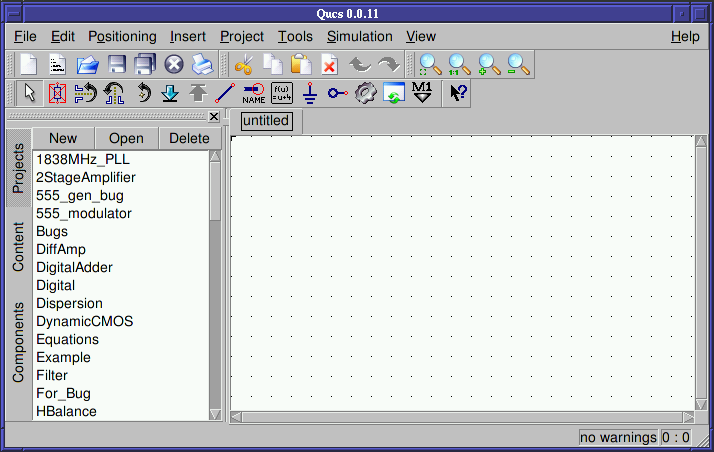
\includegraphics[width=1\linewidth]{start}
  \caption{Qucs has been started}
  \label{fig:start}
\end{figure}
\FloatBarrier

On the left hand side you find the \textbf{Projects} folder opened.
Usually the projects folder will be empty if you use Qucs for the
first time.  The large area on the right hand side is the schematic
area.  Above you can find the menu bar and the toolbars.

\medskip

In the \textbf{File} $\rightarrow$ \textbf{Application Settings} menu
the user can configure the language and appearance of Qucs.

\begin{figure}[ht]
  \centering
  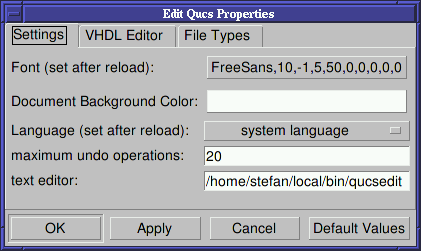
\includegraphics[width=0.6\linewidth]{appsettings}
  \caption{Application setting dialog}
  \label{fig:appsettings}
\end{figure}
\FloatBarrier

To take effect of the language and font settings the application must
be closed either via the \Ctrl+\keystroke{Q} shortcut or the
\textbf{File} $\rightarrow$ \textbf{Exit} menu entry.  Then start Qucs
again.

\tutsection{Tool suite}

Qucs consists of several standalone programs interacting with each
other through the GUI.  There are

\begin{itemize}
\item the GUI itself,

The GUI is used to create schematics, setup simulations, display
simulation results, writing VHDL code, etc.

\item the backend analogue simulator,

The analogue simulator is a command line program which is run by the
GUI in order to simulate the schematic which you previously setup.  It
takes a netlist, checks it for errors, performs the required
simulation actions and finally produces a dataset.

\item a simple text editor,

The text editor is used to display netlists and simulation logging
informations, also to edit files included by certain components
(e.g. SPICE netlists, or Touchstone files).

\item a filter synthesis application,

The program can be used to design various types of filters.

\item a transmission line calculator,

The transmission line calculator can be used to design and analyze
different types of transmission lines (e.g. microstrips, coaxial
cables).

\item a component library,

The component library manager holds models for real life devices
(e.g. transistors, diodes, bridges, opamps).  It can be extended by
the user.

\item an attenuator synthesis application,

The program can be used to design various types of passive
attenuators.

\item a command line conversion program

The conversion tool is used by the GUI to import and export datasets,
netlists and schematics from and to other CAD/EDA software.  The
supported file formats as well as usage information can be found on
the manpage of \textbf{qucsconv}.

\end{itemize}

Additionally the GUI steers other EDA tools.  For digital simulations
(via VHDL) the program FreeHDL (see \url{http://www.freehdl.seul.org})
is used.  And for circuit optimizations ASCO (see
\url{http://asco.sourceforge.net}) is configured and run.

\tutsection{Setting up schematics}

The following sections will enable the user to setup some simple
schematics.  For this we first create a new project named
``WorkBook''.  Either press the \textbf{New} button above the projects
folder or use the menu entry \textbf{Project} $\rightarrow$
\textbf{New Project} and enter the new project name.

\begin{figure}[ht]
  \centering
  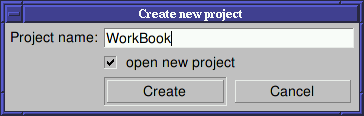
\includegraphics[width=0.6\linewidth]{newproject}
  \caption{New project dialog}
  \label{fig:newproject}
\end{figure}
\FloatBarrier

Confirm the dialog by pressing the ``Create'' button.  When done, the
project is opened and Qucs switches to the \textbf{Content} tab.

\begin{figure}[ht]
  \centering
  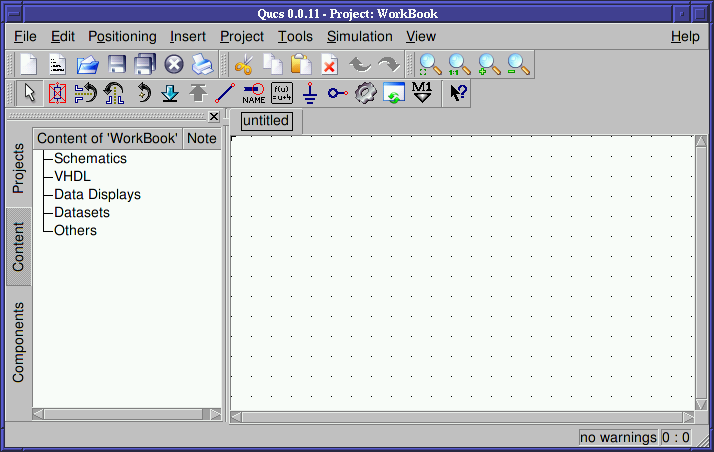
\includegraphics[width=1\linewidth]{contenttab}
  \caption{New empty project has been created}
  \label{fig:contenttab}
\end{figure}
\FloatBarrier

In the \textbf{Content} tab you will find all data related to the
project.  It contains your schematics, the VHDL files, data display
pages, datasets as well as any other data (e.g. datasheets).  On the
right hand side an ``untitled'' and empty schematic window is
displayed.

\medskip

Now you can start to edit the schematic.  The available components can
be found in the \textbf{Components} tab.

\begin{figure}[ht]
  \centering
  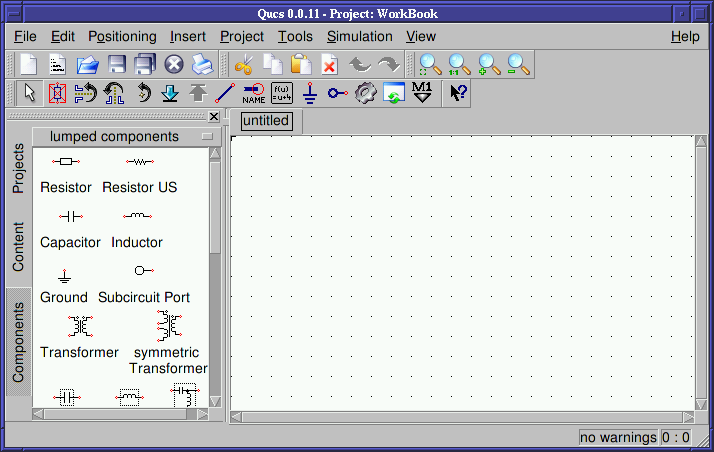
\includegraphics[width=1\linewidth]{componentstab}
  \caption{Components tab}
  \label{fig:componentstab}
\end{figure}
\FloatBarrier

In fig.~\ref{fig:componentstab} is shown when clicking the
\textbf{Components} tab.  There are lumped components (e.g. resistors,
capacitors), sources (e.g. DC and AC sources), transmission lines
(e.g. microstrip, coaxial cable, twisted pair), nonlinear components
(e.g. ideal opamp, transistors), digital components (e.g. flip-flops),
file components (e.g. Touchstone files, SPICE files), simulations
(e.g. AC or DC analysis), diagrams (e.g. cartesian or polar plot) and
paintings (e.g. texts, arrows, circles).

\medskip

Each of the components can placed on the schematic by clicking it
once, then move the mouse cursor onto the schematic and click again to
put it on its final position.  During the mouse move you can right
click in order to rotate the component into its final position.  The
user can also drag-and-drop the components.

\tutsubsection{DC simulation - A voltage divider}

The DC analysis is a steady state analysis.  It computes the node
voltage as well as branch currents of the complete circuit.  The given
circuit in fig.~\ref{fig:divider_1} is going to divide the voltage of
a DC voltage source according to the resistor ratio.

\begin{figure}[ht]
  \centering
  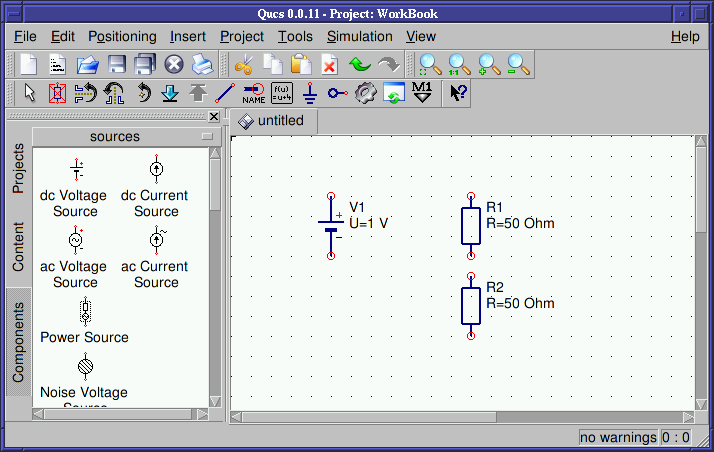
\includegraphics[width=1\linewidth]{divider_1}
  \caption{Components of the voltage divider place in the schematic area}
  \label{fig:divider_1}
\end{figure}
\FloatBarrier

\tutsubsubsection{Wiring components}

Now you need to connect the components appropriately.  This is done
using the wiring tool.  You enable the wiring mode either by clicking
the wire icon or by pressing the \Ctrl+\keystroke{E} shortcut.  Left
clicking on the components' ports (small red circles) starts a wire,
clicking on a second port finishes the wire.  In order to change the
orientation of the wire right click it.  You can leave the wiring mode
by the pressing \Esc key.

\begin{figure}[ht]
  \centering
  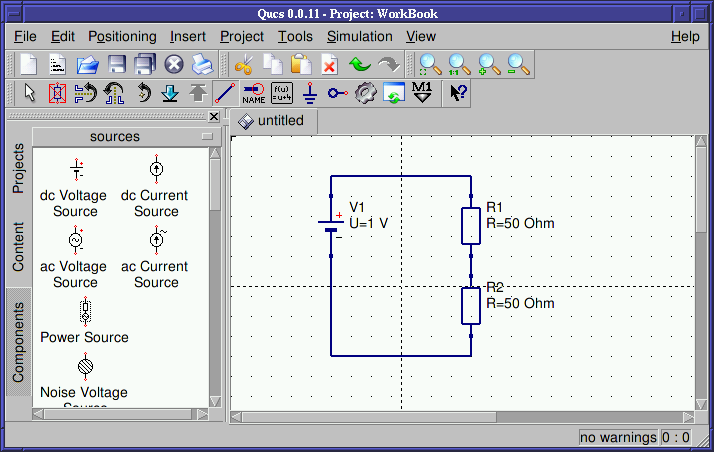
\includegraphics[width=1\linewidth]{divider_2}
  \caption{Components of the voltage divider appropriately wired}
  \label{fig:divider_2}
\end{figure}
\FloatBarrier

For any analogue simulation (including the DC simulation) there is a
reference potential required (for the nodal analysis).  The ground
symbol can be found in the \textbf{Components} tab in the
\textbf{lumped components} category.  The user can also choose the
ground symbol icon or simply press the \Ctrl+\keystroke{G} shortcut.
In the given circuit in fig.~\ref{fig:divider_3} the ground symbol is
placed at the negative terminal of the DC voltage source.

\tutsubsubsection{Placing simulation blocks}

The type of simulation which is performed must also be placed on the
schematic.  You choose the ``DC simulation'' block which can be found
in the \textbf{Components} tab in the \textbf{simulations} category.

\begin{figure}[ht]
  \centering
  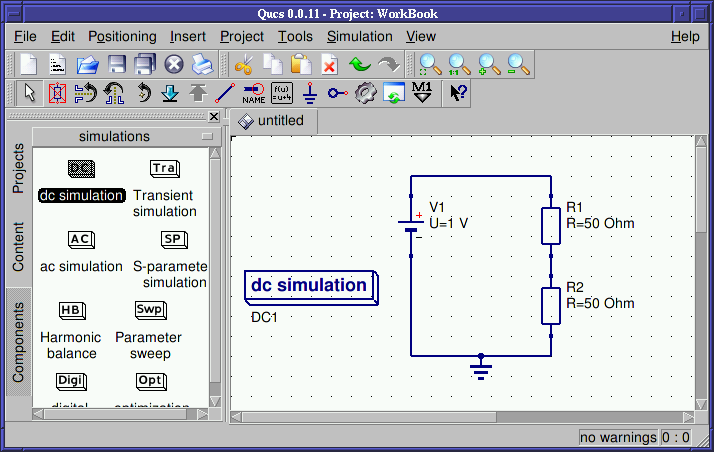
\includegraphics[width=1\linewidth]{divider_3}
  \caption{Ground symbol as well as DC simulation in place}
  \label{fig:divider_3}
\end{figure}
\FloatBarrier

\tutsubsubsection{Labelling wires}

If you want the voltage between the two resistors (the divided
voltage) be output in the dataset after simulation the user need to
label the wire.  This is done by double clicking the wire and given an
appropriate name.  Wire labelling can also be issued using the icon in
the toolbar, by pressing the \Ctrl+\keystroke{L} shortcut or by
choosing the \textbf{Insert} $\rightarrow$ \textbf{Wire Label} menu
entry.

\begin{figure}[ht]
  \centering
  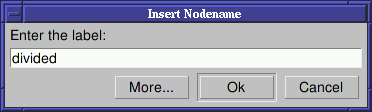
\includegraphics[width=0.6\linewidth]{nodelabel}
  \caption{Node label dialog}
  \label{fig:nodelabel}
\end{figure}
\FloatBarrier

The dialog is ended by pressing the \Enter key of pressing the ``Ok''
button.

\medskip

Now the complete schematic for the voltage divider is ready and can be
saved.  This can by achieved by choosing the \textbf{File}
$\rightarrow$ \textbf{Save} menu entry, clicking the single disk icon
or by pressing the \Ctrl+\keystroke{S} shortcut.

\begin{figure}[ht]
  \centering
  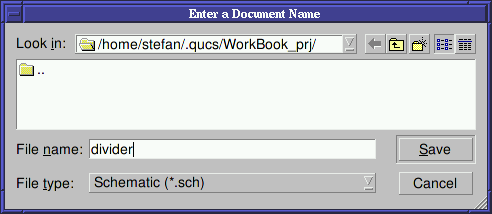
\includegraphics[width=0.7\linewidth]{divider_save}
  \caption{File save dialog}
  \label{fig:divider_save}
\end{figure}
\FloatBarrier

\begin{figure}[ht]
  \centering
  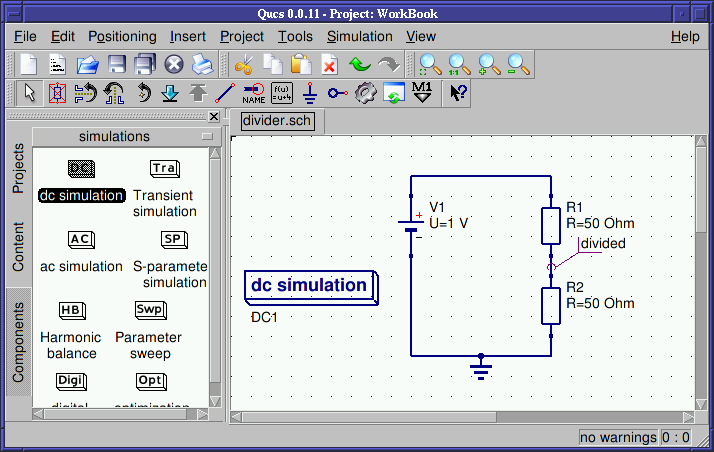
\includegraphics[width=1\linewidth]{final_divider}
  \caption{Final voltage divider schematic}
  \label{fig:final_divider}
\end{figure}
\FloatBarrier

The final DC voltage divider is shown in fig.~\ref{fig:final_divider}.

\tutsubsubsection{Issuing a simulation}

The schematic can now be simulated.  This is started by choosing the
\textbf{Simulation} $\rightarrow$ \textbf{Simulate} menu entry,
clicking the simulation button (the gearwheel) or by pressing the
\keystroke{F2} shortcut.

\begin{figure}[ht]
  \centering
  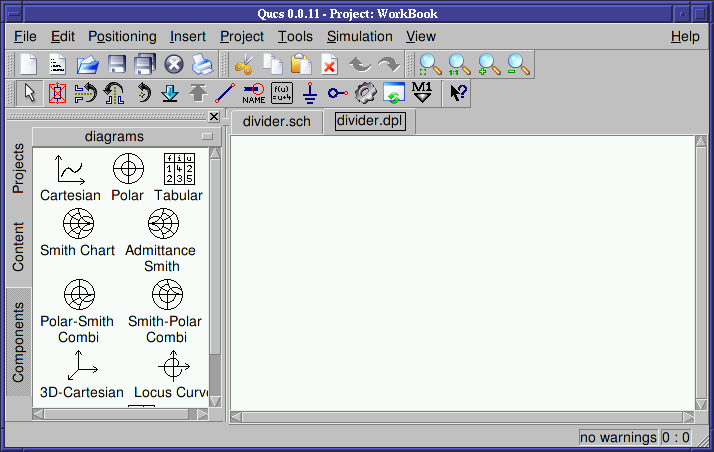
\includegraphics[width=1\linewidth]{empty_dpl}
  \caption{Empty data display after simulation finished}
  \label{fig:empty_dpl}
\end{figure}
\FloatBarrier

After the simulation has been finished the related data display is
shown (see fig.\ref{fig:empty_dpl}).  Also the \textbf{Components} tab
has changed its category to ``diagrams''.

\tutsubsubsection{Placing diagrams}

Choose the tabular (list of values) diagram and place it on the data
display page.  After dropping the tabular, the diagram dialog appears
as shown in fig.~\ref{fig:diagramdialog}.

\begin{figure}[ht]
  \centering
  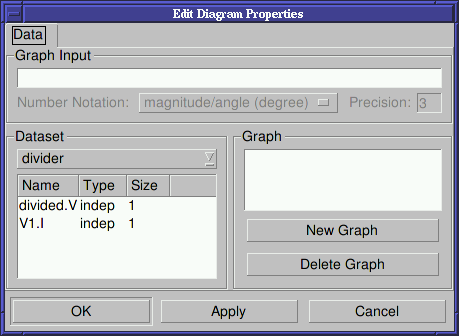
\includegraphics[width=0.7\linewidth]{diagramdialog}
  \caption{Diagram dialog}
  \label{fig:diagramdialog}
\end{figure}
\FloatBarrier

By double clicking the \textbf{divided.V} the graph (i.e. values in a
tabular plot) is added to the diagram.  Beside the node voltage
\textbf{divided.V} also the current through the DC voltage source
\textbf{V1.I} is available.  Only items listed in the dataset list can
be put into the graph.

\tutsubsubsection{Available dataset items}

Depending on the type of simulation the user performed you find the
following types of items in the dataset.
\begin{itemize}
\item \textit{node}.\textbf{V} -- DC voltage at node \textit{node}
\item \textit{name}.\textbf{I} -- DC current through component \textit{name}
\item \textit{node}.\textbf{v} -- AC voltage at node \textit{node}
\item \textit{name}.\textbf{i} -- AC current through component \textit{name}
\item \textit{node}.\textbf{vn} -- AC noise voltage at node \textit{node}
\item \textit{name}.\textbf{in} -- AC noise current through component \textit{name}
\item \textit{node}.\textbf{Vt} -- transient voltage at node \textit{node}
\item \textit{name}.\textbf{It} -- transient current through component \textit{name}
\item \textit{S[1,1]} -- S-parameter value
\end{itemize}

Please note that all voltages and currents are peak values and all
noise voltages are RMS values at 1Hz bandwidth.

\begin{figure}[ht]
  \centering
  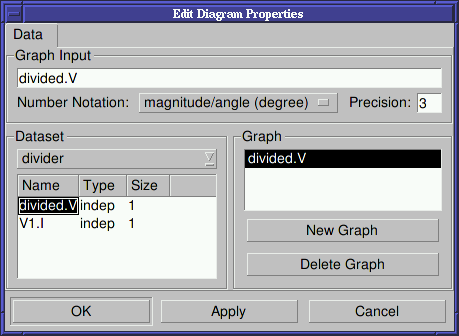
\includegraphics[width=0.7\linewidth]{diagramdialog_divided}
  \caption{Diagram dialog with the node voltage added}
  \label{fig:diagramdialog_divided}
\end{figure}
\FloatBarrier

Depending on the type of graph you have various options to choose for
the graph.  For a tabular graph there is the the number precision as
well as type of number notation (important for complex values).  Press
the ``Ok'' button to close the dialog.

\begin{figure}[ht]
  \centering
  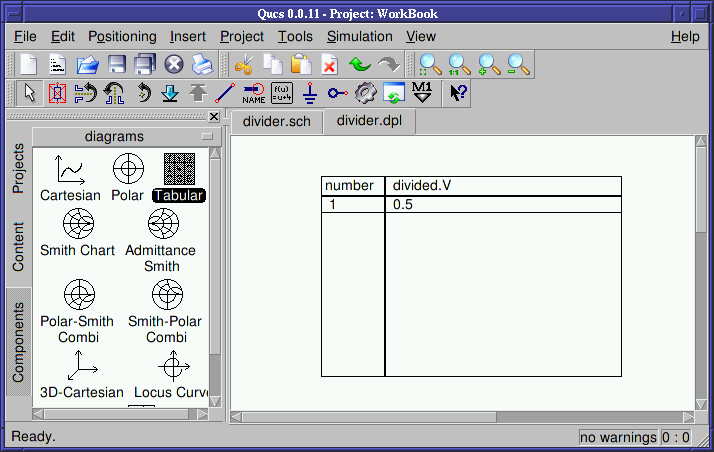
\includegraphics[width=1\linewidth]{divided_dpl}
  \caption{Data display with tabular graph}
  \label{fig:divided_dpl}
\end{figure}
\FloatBarrier

In the tabular graph you see now the value of the node voltage
\textbf{divided.V} which is 0.5V.  That was expected since the values
of the resistors are equally sized and the DC voltage source produces
1V.

\medskip

Congratulations! You made your first successful simulation using Qucs.

\tutsubsubsection{Changing component properties}

If you want to change the resistor ratio then switch back to your
schematic either by clicking on the \textbf{divider.sch} tab, by
pressing the \keystroke{F4} shortcut or by choosing the
\textbf{Simulation} $\rightarrow$ \textbf{View Data Display/Schematic}
menu entry.  Afterwards double click the \textbf{R1} resistor.  This
opens the component property dialog shown in
fig.~\ref{fig:componentprops}.

\begin{figure}[ht]
  \centering
  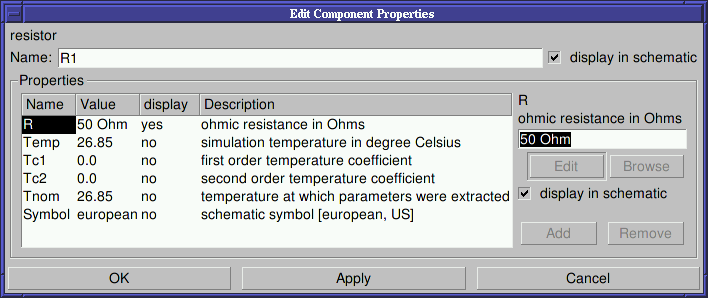
\includegraphics[width=1\linewidth]{componentprops}
  \caption{Component property dialog for the R1 resistor}
  \label{fig:componentprops}
\end{figure}
\FloatBarrier

In the component property dialog all the properties of a given
component can be edited.  A short description is given as well as
there is a checkbox for each property \textbf{display in schematic}
which can be used to add the property name and value on the schematic
(or to hide it).

\tutparagraph{Allowed property values}

For component values either standard (1000), scientific (1e-3) or an
engineering (1k) number notation can be chosen.  Some units are also
allowed.  The units are
\begin{itemize}
\item Ohm -- resistance / $\Omega$
\item s -- time / Seconds
\item S -- conductance / Siemens
\item K -- temperature / Kelvin
\item H -- inductance / Henry
\item F -- capacitance / Farad
\item Hz -- frequency / Hertz
\item V -- voltage / Volt
\item A -- current / Ampere
\item W -- power / Watt
\item m -- length / Meter (not usable standalone, see paragraph below)
\end{itemize}

The available engineering suffixes are
\begin{itemize}
\item dBm -- $\mathrm{10\cdot\log{\left(x/0.001\right)}}$
\item dB -- $\mathrm{10\cdot\log{\left(x\right)}}$
\item T -- $10^{12}$
\item G -- $10^{9}$
\item M -- $10^{6}$
\item k -- $10^{3}$
\item m -- $10^{-3}$
\item u -- $10^{-6}$
\item n -- $10^{-9}$
\item p -- $10^{-12}$
\item f -- $10^{-15}$
\item a -- $10^{-18}$
\end{itemize}

Please note that all units and engineering suffixes are \textbf{case
sensitive} and also note the conflict in \textbf{m}.  When specifying
one millimeter you can use 1mm.  One meter (1m) cannot be specified
and will always be interpreted as one milli (engineering notation).

\medskip

Now you can change the resistor value to $1\Omega$, see
fig.~\ref{fig:componentprops_1}.

\begin{figure}[ht]
  \centering
  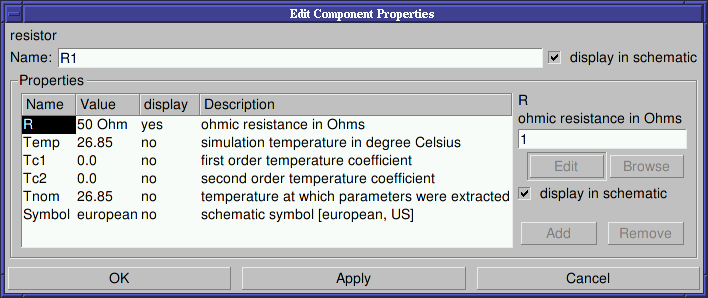
\includegraphics[width=1\linewidth]{componentprops_1}
  \caption{Component property dialog for the R1 resistor}
  \label{fig:componentprops_1}
\end{figure}
\FloatBarrier

Press the ``OK'' button to close the dialog.  You will get the
following schematic.

\begin{figure}[ht]
  \centering
  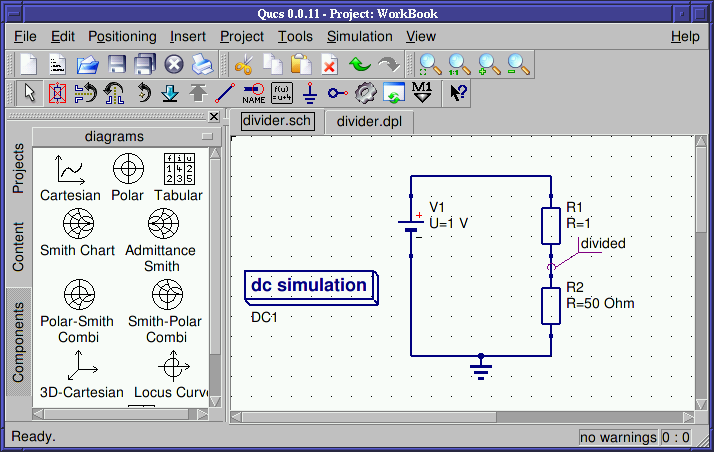
\includegraphics[width=1\linewidth]{divider_4}
  \caption{Value of resistor \textbf{R1} changed}
  \label{fig:divider_4}
\end{figure}
\FloatBarrier

In order to change the value of the resistor \textbf{R2} you can just
click on the \textbf{50 Ohm} value directly on the schematic and edit
the value.

\begin{figure}[ht]
  \centering
  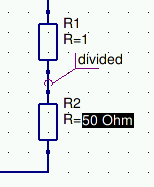
\includegraphics[width=0.2\linewidth]{propdirect}
  \caption{Change value of resistor \textbf{R2} directly on schematic}
  \label{fig:propdirect}
\end{figure}
\FloatBarrier

Change the value to ``3'' which will give a resistor ratio of $3/(1+3)
= 0.75$.  Now you have the following schematic.

\begin{figure}[ht]
  \centering
  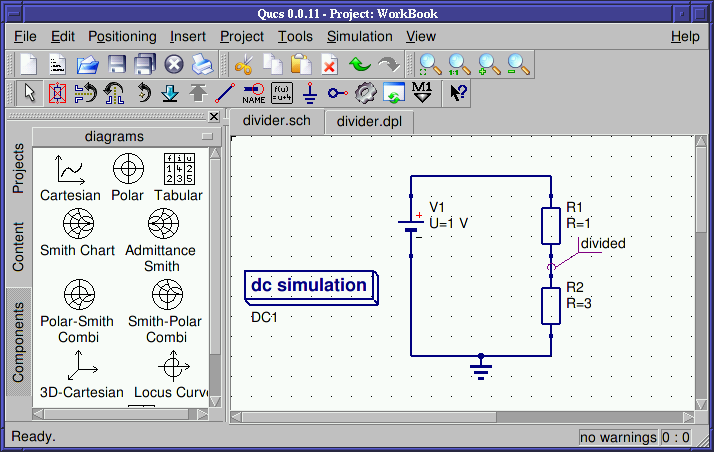
\includegraphics[width=1\linewidth]{divider_5}
  \caption{Value of resistor \textbf{R2} changed}
  \label{fig:divider_5}
\end{figure}
\FloatBarrier

Diagrams are not limited to be placed on the data display, they can
also reside on the schematic directly.  Thus you can place again now a
tabular diagram on the schematic and add the \textbf{divided.V} value.
The diagram will show the result from the previous simulation.

\tutsubsubsection{Changing document properties}

If you do not want Qucs to change automatically to the associated data
display you can change the behaviour in the document setting dialog.
You can go to the document settings dialog by right clicking on free
space on the schematic area and choose the \textbf{Document Settings}
menu item in the context menu which pops up or by choosing the
\textbf{File} $\rightarrow$ \textbf{Document Settings} menu entry.

\begin{figure}[ht]
  \centering
  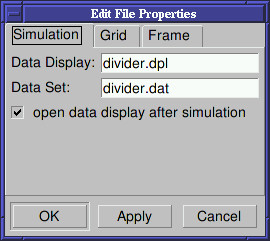
\includegraphics[width=0.4\linewidth]{fileprops}
  \caption{Document settings dialog}
  \label{fig:fileprops}
\end{figure}
\FloatBarrier

In the dialog you uncheck the \textbf{open data display after
simulation} item.  Press the ``OK'' button to apply the change.  If
you now resimulate the schematic by pressing the \keystroke{F2}
shortcut the ``Qucs Simulation Messages'' dialog window opens and can
be left by pressing \Esc.  The tabular diagram now show the new value
for \textbf{divided.V}.

\begin{figure}[ht]
  \centering
  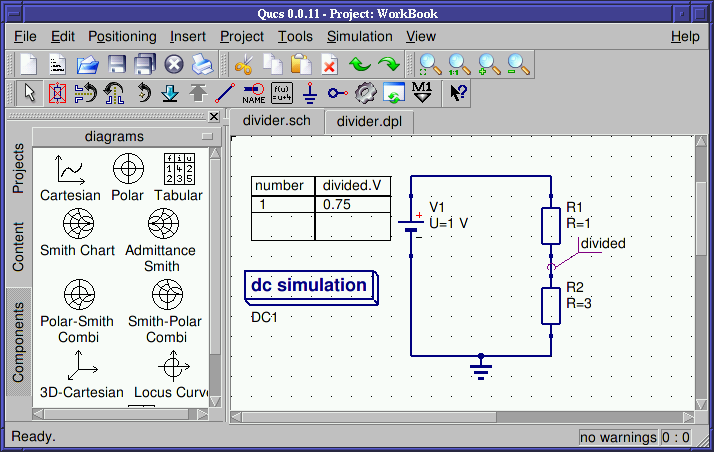
\includegraphics[width=1\linewidth]{divider_6}
  \caption{Divider schematic after new simulation}
  \label{fig:divider_6}
\end{figure}
\FloatBarrier

\tutsubsection{DC simulation - Characteristics of a transistor}

We are now going ahead and will setup schematics for some
characteristic curves of a bipolar transistor using DC simulation and
the parameter sweep.

\begin{figure}[ht]
  \centering
  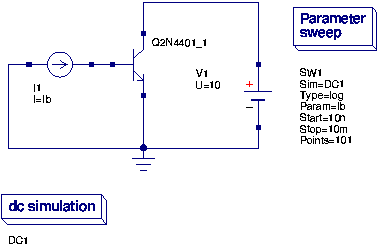
\includegraphics[width=0.7\linewidth]{igain_1}
  \caption{Swept DC simulation setup}
  \label{fig:igain_1}
\end{figure}
\FloatBarrier

In the schematic in fig.~\ref{fig:igain_1} there is a bipolar
transistor placed in a common emitter configuration.  Additionally a
parameter sweep has been placed.  Please note the \textbf{Sim}
property of the parameter sweep.  It contains the instance name of the
DC simulation \textbf{DC1} which is going to be swept.  The parameter
which is swept is \textbf{Ib} (the base current) and is put into the
\textbf{Param} property of the parameter sweep.  The parameter
\textbf{Ib} is also put into the \textbf{I} property of the DC current
source \textbf{I1}.

\tutsubsubsection{Using the component library}

The bipolar transistor has been taken from the component library.  You
can start the program by choosing the \textbf{Tools} $\rightarrow$
\textbf{Component Library} menu entry or by pressing the
\Ctrl+\keystroke{4} shortcut.

\begin{figure}[ht]
  \centering
  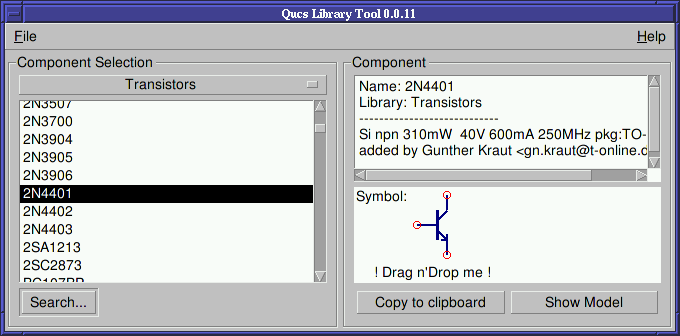
\includegraphics[width=1\linewidth]{componentlibrary}
  \caption{Component library tool}
  \label{fig:componentlibrary}
\end{figure}
\FloatBarrier

When choosing the ``Transistor'' category with the combobox you find
the ``2N4401'' transistor.  By clicking the ``Copy to clipboard''
button the component is available in the clipboard and can be inserted
in the schematic using the \Ctrl+\keystroke{V} shortcut or by choosing
the \textbf{Edit} $\rightarrow$ \textbf{Paste} menu entry.  The
component can also by dragged onto the schematic by clicking on the
symbol in the library tool.

\medskip

So what do we want to simulate actually?  It is the current transfer
curve of the bipolar transistor.  The input current (at the base) is
given by the swept parameter \textbf{Ib}.  The output current (at the
collector) flows through the DC voltage source \textbf{V1}.  The
current transfer curve is:
\begin{equation*}
\beta_{DC} = f\left(I_C\right) = I_C / I_B
\end{equation*}

The current through the voltage source \textbf{V1} is the collector
current flowing out of the transistor.

\tutsubsubsection{Placing equations on the schematic}

In order to compute the necessary values for the transfer curve we
need to place some equations on the schematic.  This is done by
clicking the equation icon or by choosing the \textbf{Insert}
$\rightarrow$ \textbf{Insert Equation} menu entry.  When double
clicking the equation component you can edit the equations to be
computed.

\begin{figure}[ht]
  \centering
  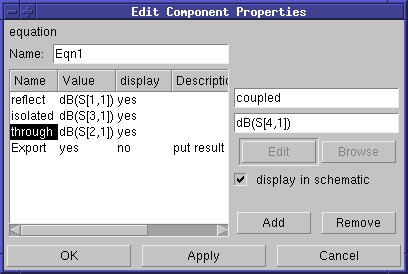
\includegraphics[width=0.6\linewidth]{eqndialog}
  \caption{Equation dialog}
  \label{fig:eqndialog}
\end{figure}
\FloatBarrier

In the upper edit box you enter the name of the equation and in the
lower one the computation formula.  The resulting schematic is shown
in fig.~\ref{fig:igain_2}.

\begin{figure}[ht]
  \centering
  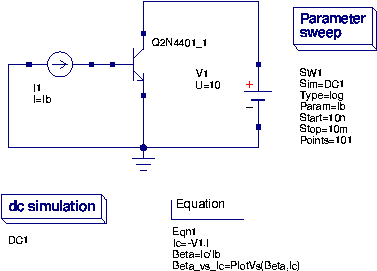
\includegraphics[width=0.7\linewidth]{igain_2}
  \caption{Swept DC simulation setup with equations}
  \label{fig:igain_2}
\end{figure}
\FloatBarrier

Note that three equations have been added.  The first one
\textbf{Ic=-V1.I} is the collector current flowing into the transistor
(current though voltage sources flow from the positive terminal to the
negative terminal).  The equation \textbf{Beta=Ic/Ib} computes the
current gain and finally \textbf{Beta\_vs\_Ic=PlotVs(Beta,Ic)} changes
the data dependency of the current gain to be the collector current.
The original data dependency is the swept parameter \textbf{Ib}.

\tutsubsubsection{The internal help system}

The full list of available functions in the equation solver can be
seen in the internal help system.  It is started by pressing the
\keystroke{F1} shortcut or by choosing the \textbf{Help} $\rightarrow$
\textbf{Help Index} menu entry.  In the sidebar choose the ``Short
Description of mathematical Functions'' entry.

\begin{figure}[ht]
  \centering
  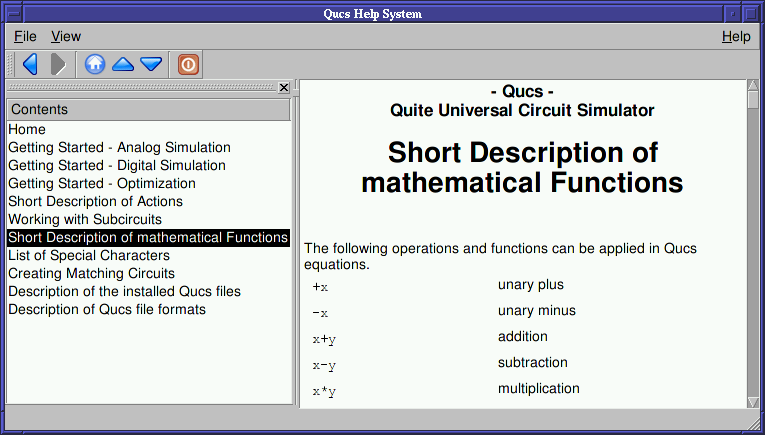
\includegraphics[width=1\linewidth]{helpdialog}
  \caption{Internal help system}
  \label{fig:helpdialog}
\end{figure}
\FloatBarrier

The help can be closed using the \Ctrl+\keystroke{Q} shortcut.

\tutsubsubsection{Configuring cartesian diagrams}

In fig.~\ref{fig:igain_3} the final simulation result is shown.  In
the diagram dialog the \textbf{Beta\_vs\_Ic} dataset entry was chosen.

\begin{figure}[ht]
  \centering
  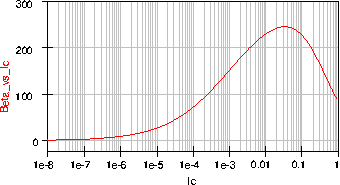
\includegraphics[width=0.6\linewidth]{igain_3}
  \caption{Simulation result}
  \label{fig:igain_3}
\end{figure}
\FloatBarrier

Additionally the x-axis has been chosen to be logarithmic.  The
x-axis label is \textbf{Ic}.

\begin{figure}[ht]
  \centering
  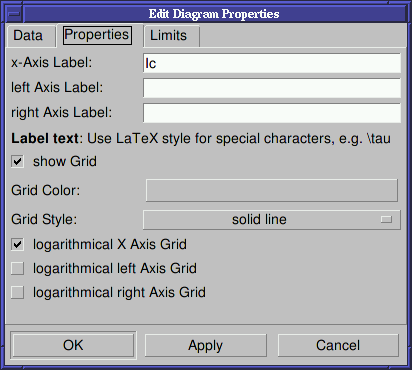
\includegraphics[width=0.6\linewidth]{diagramdialog_1}
  \caption{Editing diagram properties}
  \label{diagramdialog_1}
\end{figure}
\FloatBarrier

\tutsubsubsection{Working with markers in diagrams}

The current gain curve in diagram in fig.~\ref{fig:igain_3} shows a
maximum value.  If you want to know the appropriate values it is
possible to use markers for this purpose.

\begin{figure}[ht]
  \centering
  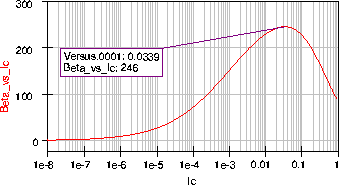
\includegraphics[width=0.6\linewidth]{igain_4}
  \caption{Cartesian diagram with marker}
  \label{fig:igain_4}
\end{figure}
\FloatBarrier

This is achieved by pressing the \Ctrl+\keystroke{B} shortcut,
clicking the marker icon or choosing the \textbf{Insert} $\rightarrow$
\textbf{Set Marker on Graph} menu entry.  Then click on the diagrams
curve you want to have the marker at.  If the marker is selected you
can move it by pressing the arrow keys \LArrow, \RArrow and \UArrow or
\DArrow for multi-dimensional graphs.

\begin{figure}[ht]
  \centering
  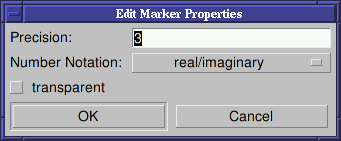
\includegraphics[width=0.5\linewidth]{markerdialog}
  \caption{Marker dialog}
  \label{fig:imarkerdialog}
\end{figure}
\FloatBarrier

Double clicking the marker opens the marker dialog.  There you can
configure the precision as well as the number notation of the
displayed values.

\tutsubsubsection{A multi-dimensional sweep}

Now we are going to create a schematic for the output characteristics
of the bipolar transistor.  The characteristic curve is defined as
follows:
\begin{equation*}
I_{C} = f\left(I_B, V_{CE}\right)
\end{equation*}

Thus it is necessary to modify the schematic from the previous
sections a bit.

\begin{figure}[ht]
  \centering
  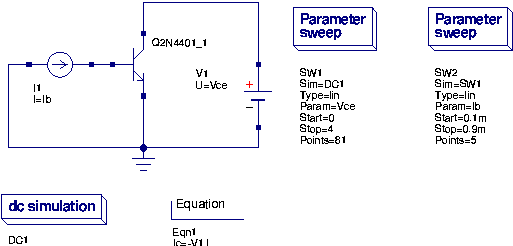
\includegraphics[width=0.8\linewidth]{outputbjt_1}
  \caption{Sweep setup for the output characteristics}
  \label{fig:outputbjt_1}
\end{figure}
\FloatBarrier

A second parameter sweep has been added.  The first order sweep is
\textbf{Vce} specified in the parameter sweep \textbf{SW1}.  The
\textbf{Sim} parameter points to the instance name of the DC
simulation \textbf{DC1}.  The second order sweep is \textbf{Ib}
specified in the parameter sweep \textbf{SW2}. The \textbf{Sim}
parameter of this second sweep points to the instance name of the
first sweep \textbf{SW1}.  The first order sweep variable \textbf{Vce}
is put into the \textbf{U} property of the DC voltage source
\textbf{V1}.

\begin{figure}[ht]
  \centering
  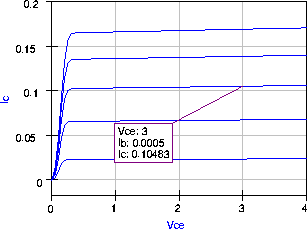
\includegraphics[width=0.6\linewidth]{outputbjt_2}
  \caption{Output characteristics of a NPN bipolar transistor}
  \label{fig:outputbjt_2}
\end{figure}
\FloatBarrier

\tutsubsection{AC simulation - Transit frequency of a bipolar transistor}

In the next section we are going to determine the transit frequency of
the bipolar transistor used in the previous DC sections.  First a bias
point is chosen.  In fig.~\ref{fig:igain_beta_1} the DC setup was a
bit modified.

\begin{figure}[ht]
  \centering
  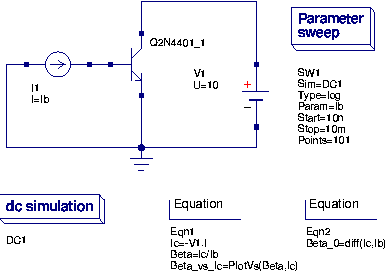
\includegraphics[width=0.6\linewidth]{igain_beta_1}
  \caption{DC setup for determining a bias point for AC simulation}
  \label{fig:igain_beta_1}
\end{figure}
\FloatBarrier

There is now an additional equation computing the RF current gain for
zero frequency which is \textbf{Beta\_0=diff(Ic,Ib)}.  The equation
denotes
\begin{equation*}
\beta_{RF}\left(f=0\right) = \dfrac{\partial Ic}{\partial Ib}
\end{equation*}

In fig.~\ref{fig:igain_ib} the DC current gain from
fig.~\ref{fig:igain_4} is plotted versus the base current \textbf{Ib}
choosing \textbf{Beta} in the diagram dialog instead of
\textbf{Beta\_vs\_Ic}.  The appropriate base current shown in the
marker is $140\micro\ampere$.

\begin{figure}[ht]
  \centering
  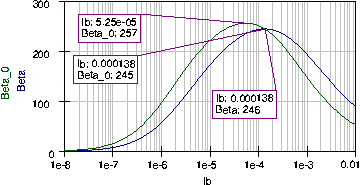
\includegraphics[width=0.6\linewidth]{igain_ib}
  \caption{DC current gain vs. base current}
  \label{fig:igain_ib}
\end{figure}
\FloatBarrier

It can be seen that the maximum AC current gain (257 @
$53\micro\ampere$) differs from the maximum DC gain.  Also the AC
current gain almostly equals the DC current gain at the base current
for the maximum DC current gain.  For maximum RF performance the base
current with the maximum AC current gain could be chosen.  But there
may be other consideration, e.g. DC power dissipation, so we choose
the bias point with the maximum DC current gain -- arbitrarily.

\begin{figure}[ht]
  \centering
  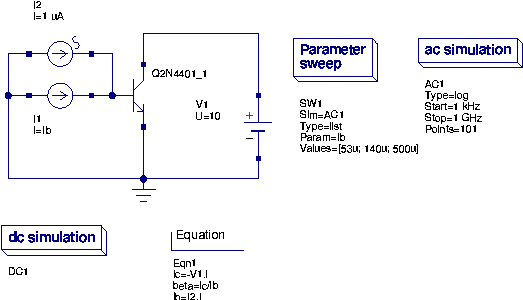
\includegraphics[width=0.85\linewidth]{bjtac_1}
  \caption{Bias dependent AC simulation setup}
  \label{fig:bjtac_1}
\end{figure}
\FloatBarrier

In fig.~\ref{fig:bjtac_1} is a DC bias dependent AC simulation setup
shown.  The DC base current \textbf{Ib} is swept for
$53\micro\ampere$, $140\micro\ampere$ and $500\micro\ampere$.
Additionally the AC simulation block has been placed on the schematic.

\medskip

The \textbf{Sim} parameter of the \textbf{SW1} parameter sweep is set
to the instance name of the AC simulation \textbf{AC1}.  Qucs
automatically ``knows'' that the DC simulation has to be run before
each AC simulation since it is required to determine the appropriate
bias points.

\medskip

The AC current current source \textbf{I2} is in parallel to the DC
current source and has an AC amplitude of $1\micro\ampere$.  During
the AC simulation the DC current source \textbf{I1} is an ideal open
and the DC voltage source \textbf{V1} is an ideal short.

\medskip

In the equations \textbf{V1.i} (mark the small i letter) denotes the
AC current through the DC voltage source \textbf{V1}.  The AC base
current \textbf{ib} is taken from the input parameter \textbf{I2.I}
denoting the value of the property \textbf{I} of the AC current source
\textbf{I2} ($1\micro\ampere$).

\medskip

After pressing \keystroke{F2} -- to start the simulation -- the
following cartesian diagram can be placed on the data display page,
see fig.~\ref{fig:bjtac_2}.

\begin{figure}[ht]
  \centering
  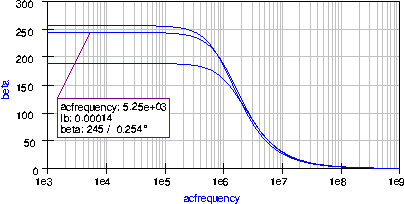
\includegraphics[width=0.7\linewidth]{bjtac_2}
  \caption{AC current gain of the bipolar transistor}
  \label{fig:bjtac_2}
\end{figure}
\FloatBarrier

The marker clearly shows for the low frequency range ($f \rightarrow
0$) the DC current gain of 246 (for $I_B = 140\micro\ampere$) which
was already determined in fig.~\ref{fig:igain_ib}.

\medskip

In the next AC simulation setup shown in fig.~\ref{fig:bjtacft_1} the
parameter sweep is dropped to concentrate on the determination of the
transit frequency.  The transit frequency of a bipolar transistor
denotes the frequency where the AC current gain drops to 1 (0 dB).
\begin{equation*}
f_T \; \leftarrow \; \left|h_{21}\right|^2 = 1
\end{equation*}

Expressed in h-parameters of a general two-port the AC current gain
is:
\begin{equation*}
\beta_{RF} = h_{21} = \left.\dfrac{i_2}{i_1}\right|_{v_2=0}
\end{equation*}

whereas port 1 is the base and port 2 the collector.  The side
condition ($v_2=0$) is given in our setup since the DC voltage source
is an ideal AC short.

\begin{figure}[ht]
  \centering
  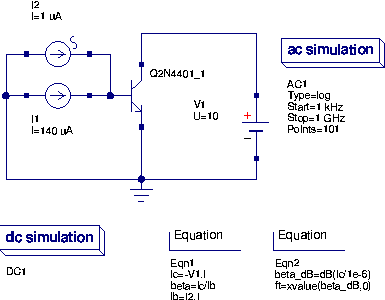
\includegraphics[width=0.6\linewidth]{bjtacft_1}
  \caption{AC setup for determining the transit frequency}
  \label{fig:bjtacft_1}
\end{figure}
\FloatBarrier

There are two more equations in the setup.  One calculates the AC
current gain in dB (which is $\mathrm{20\cdot\log{\left(beta\right)}}$
and the other one is \textbf{ft=xvalue(beta\_dB,0)}.  The equation
searches for the nearest given x-value (in this case the frequency)
where \textbf{beta\_dB} approaches \textbf{0}.

\begin{figure}[ht]
  \centering
  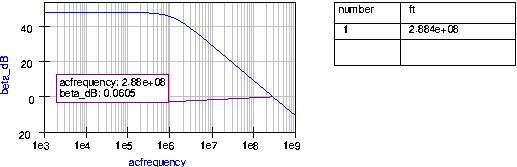
\includegraphics[width=0.9\linewidth]{bjtacft_2}
  \caption{Bode plot of the current transfer function}
  \label{fig:bjtacft_2}
\end{figure}
\FloatBarrier

In fig.~\ref{fig:bjtacft_2} the Bode plot (double logarithmic plot) of
the current transfer function of the bipolar transistor is shown.  The
current gain is constant up to the corner frequency and then drops by
20dB/decade.  The marker finally denotes where the gain is finally
0dB.  The equation for \textbf{ft} worked correctly as seen in the
beside tabular.  The transit frequency of the bipolar transistor in
this bias point is approximately $288\mega\hertz$.

\tutsubsection{AC simulation - A simple RC highpass}

Simple circuit AC analysis (circuit frequency response analysis) can
be carried out easily by using the \emph{AC Simulation} block.

\addvspace{12pt}

For instance, a simple high pass RC filter can be analyzed by
constructing first the schematic displayed on
figure~\ref{fig:highpassrc} which corresponds to a high pass RC
network.

\begin{figure}[ht]
  \centering
  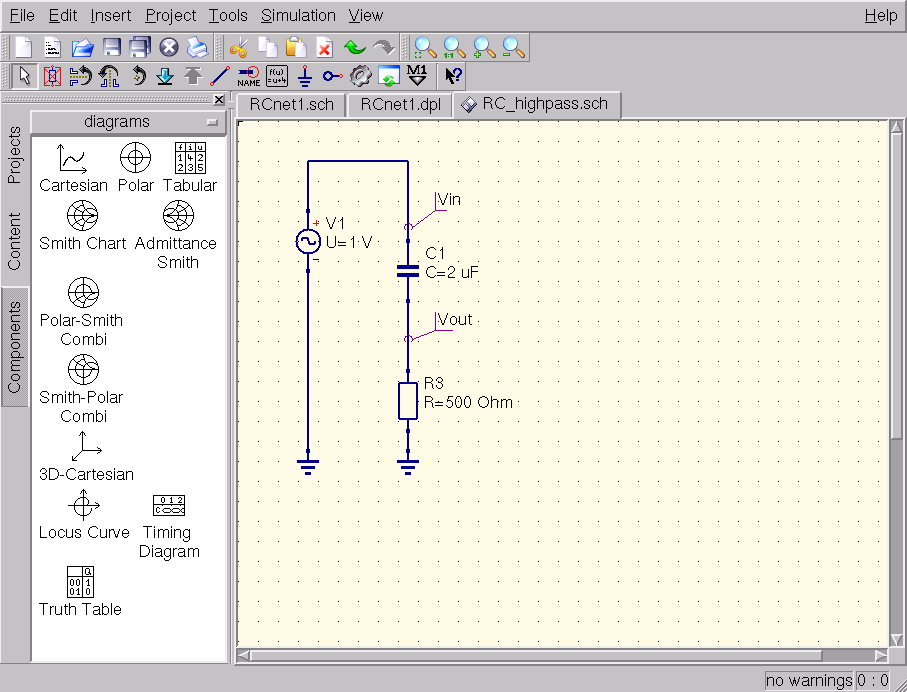
\includegraphics[width=1\linewidth]{highpassrc}
  \caption{simple RC high-pass filter schematic}
  \label{fig:highpassrc}
\end{figure}
\FloatBarrier

Performing the actual AC analysis is as easy as dragging and dropping an
\emph{AC Simulation} block available under the \emph{Simulations}
tab as can be seen in figure~\ref{fig:highpassimblock}. 

\begin{figure}[ht]
  \centering
  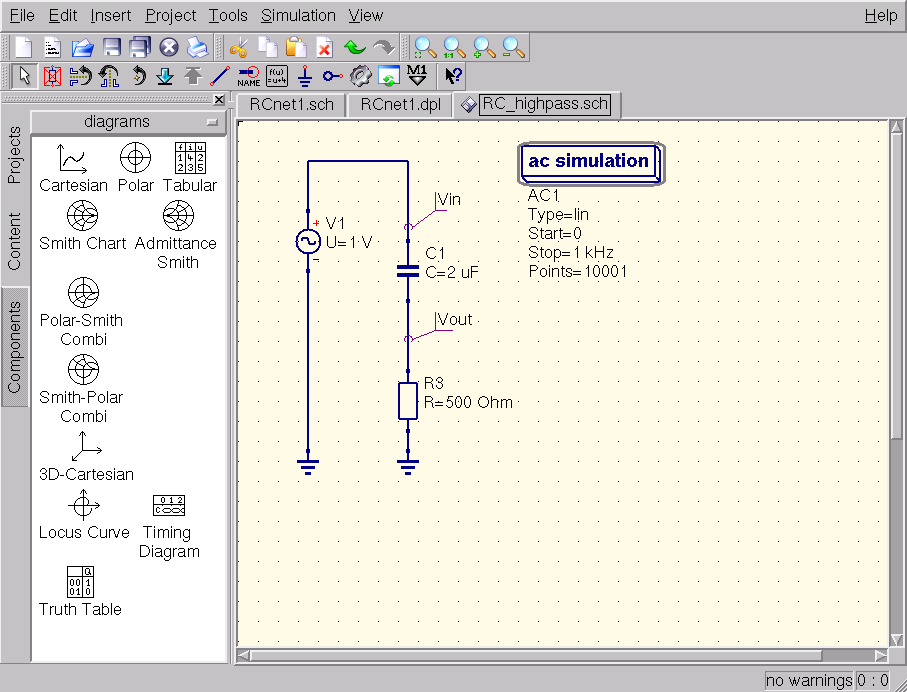
\includegraphics[width=0.75\linewidth]{highpasssimblock}
  \caption{AC simulation block placed}
  \label{fig:highpassimblock}
\end{figure}
\FloatBarrier

Once this is done one must configure the ranges of the simulation
analysis by clicking twice on the \emph{AC Simulation} box as can be
seen in figure~\ref{fig:simblockconfig}.

\begin{figure}[ht]
  \centering
  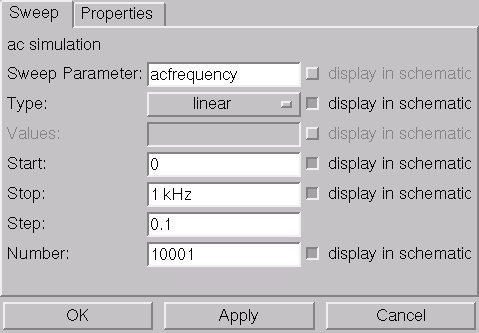
\includegraphics[width=0.45\linewidth]{simblockconfig}
  \caption{AC simulation block configuration dialog}
  \label{fig:simblockconfig}
\end{figure}
\FloatBarrier

Finally by pressing \keystroke{F2} the simulation takes places and a graphic
report can be generated by selecting the right plot as seen in the
previous sections. The final view of the network with its respective
frequency analysis can be seen on figure~\ref{fig:finalhighpassrc}.

\begin{figure}[ht]
  \centering
  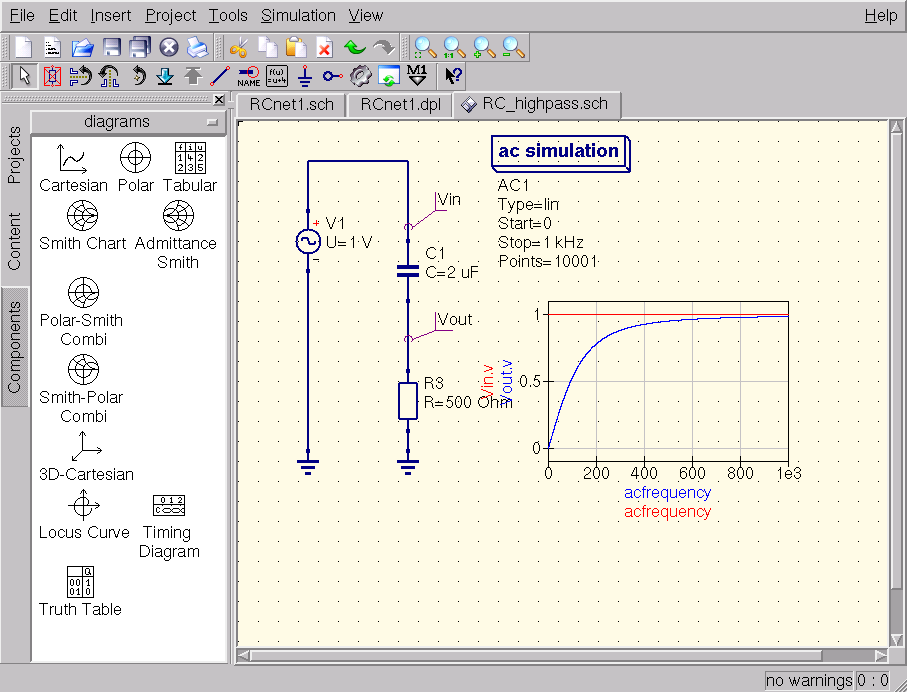
\includegraphics[width=1\linewidth]{finalhighpassrc}
  \caption{AC simulation results}
  \label{fig:finalhighpassrc}
\end{figure}
\FloatBarrier

\tutsubsection{Transient simulation - Amplification of a bipolar transistor}

Based on the schematic in fig.~\ref{fig:bjtacft_1} we are now going to
simulate the bipolar transistor in the time domain.

\begin{figure}[ht]
  \centering
  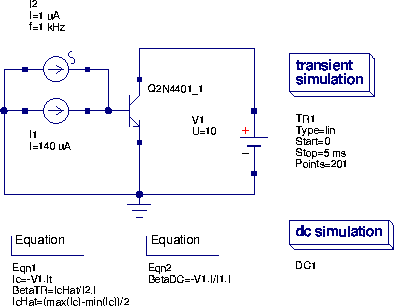
\includegraphics[width=0.7\linewidth]{bjttr_1}
  \caption{Transient simulation setup}
  \label{fig:ibjttr_1}
\end{figure}
\FloatBarrier

As shown in fig.~\ref{fig:ibjttr_1} the transient simulation block was
placed on the schematic.  Also the frequency \textbf{f} of the AC
current source \textbf{I2} was set to 1kHz.  The start time of the
transient simulation is set to 0 and the stop time to 5ms which will
include 5 periods of the input signal.

\medskip

The additional DC simulation block is not necessary for the transient
simulation but left there for some result comparison.

\medskip

The collector current in the equations is denoted by the transient
current \textbf{-V1.It}.  The peak value if the collector current is
determined by the equation for \textbf{IcHat}.  The current gain
during transient simulation is calculated using
\textbf{BetaTR=IcHat/I2.I} whereas \textbf{I2.I} denotes the component
property \textbf{I} of the the current source \textbf{I2} (which is
$1\micro\ampere$ peak).  The current gain \textbf{BetaDC} is computed
for convenience.

\medskip

The equation blocks imply that the order of appearance of assignments
does not matter (e.g. \textbf{IcHat} is used before computed).  The
equation solver will take care of such dependencies.

\begin{figure}[ht]
  \centering
  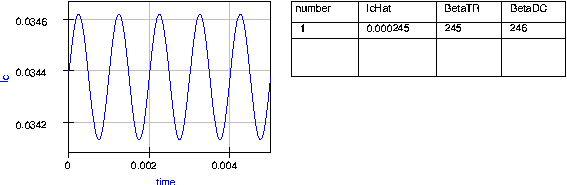
\includegraphics[width=1\linewidth]{bjttr_2}
  \caption{Transient results}
  \label{fig:ibjttr_2}
\end{figure}
\FloatBarrier

Fig.~\ref{fig:ibjttr_2} shows the results of the transient as well as
DC simulation.  The time dependent collector current oscillates around
its bias point.  The current gain of the transient signal corresponds
perfectly with the DC value.  That is because a rather small frequency
of 1kHz was chosen.

\tutsubsection{S-parameter simulation - Transit frequency of a BJT}

In the following section the S-parameter simulation is introduced.
The S-parameter simulation is -- similar to the AC simulation -- a
small signal analysis in the frequency domain.

\begin{figure}[ht]
  \centering
  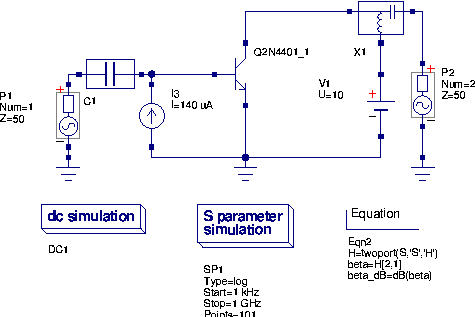
\includegraphics[width=0.8\linewidth]{bjtsp_1}
  \caption{S-parameter simulation setup for the bipolar transistor}
  \label{fig:bjtsp_1}
\end{figure}
\FloatBarrier

Similar to the AC setup in fig.~\ref{fig:bjtacft_1} the S-parameter
setup in fig.~\ref{fig:bjtsp_1} uses the same biasing.  The setup will
be used to determine the transit frequency of the bipolar transistor.

\medskip

The two AC power sources \textbf{P1} and \textbf{P2} are required for
a two-port S-parameter simulation.  They can be found in the
\textbf{Components} tab in the \textbf{sources} category.  Depending
on the number of these kind of sources one-port, two-port and
multi-port simulations are performed.  The \textbf{Num} property of
the sources determines the location of the matrix entries in the
resulting S-parameter matrix.  The \textbf{Z} properties define the
reference impedance of the S-parameters.

\medskip

The additional DC block \textbf{C1} at the base node and the bias tee
\textbf{X1} on the collector is used to decouple the signal path of
the biasing DC sources from the internal impedance of the AC power
sources.  Also the bias tee ensures that the AC signal from the
\textbf{P2} source is not shorted by the DC source \textbf{V1}.  The
same functionality is achieved by the DC current source \textbf{I3} at
the base.  It represents an ideal AC open.

\medskip

The S-parameter simulation itself is selected by placing the
S-parameter block \textbf{SP1} on the schematic.  The same frequency
range is chosen as in the previous AC simulations.

\medskip

The equations contain a two-port conversion function which convert the
resulting S-parameter \textbf{S} into the appropriate H-parameters
\textbf{H}.  Again the AC current gain $\mathrm{h_{21}}$ is calculated
and converted in dB.

\begin{figure}[ht]
  \centering
  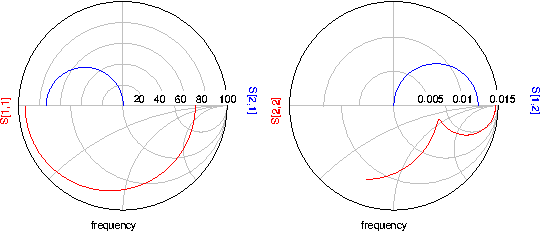
\includegraphics[width=1\linewidth]{bjtsp_3}
  \caption{S-parameters of the bipolar transistor}
  \label{fig:bjtsp_3}
\end{figure}
\FloatBarrier

In fig.~\ref{fig:bjtsp_3} the four complex S-parameters are displayed
in two \textbf{Polar-Smith Combi} diagrams.  They represent what can
be expected from a typical bipolar transistor.

\medskip

Using the computed H-parameters we can now compare the S-parameter
simulation results with those of the AC simulation.
Fig.~\ref{fig:bjtsp_2} shows that the curves \textbf{beta\_dB} of both
simulation setups cover perfectly each other.  Again the transit
frequency is approximately 288MHz.

\begin{figure}[ht]
  \centering
  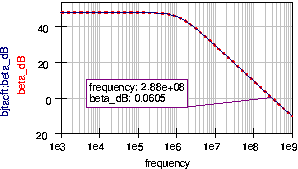
\includegraphics[width=0.65\linewidth]{bjtsp_2}
  \caption{Comparison between S-parameter and AC result}
  \label{fig:bjtsp_2}
\end{figure}
\FloatBarrier

The diagram implies that you can compare data curves from different
setups.  This is indicated by the \textbf{bjtacft:} prefix.  The
appropriate dataset file \textbf{bjtacft.dat} can be selected in the
diagram dialog as shown in fig.~\ref{fig:diagramdialog_sets}.

\begin{figure}[ht]
  \centering
  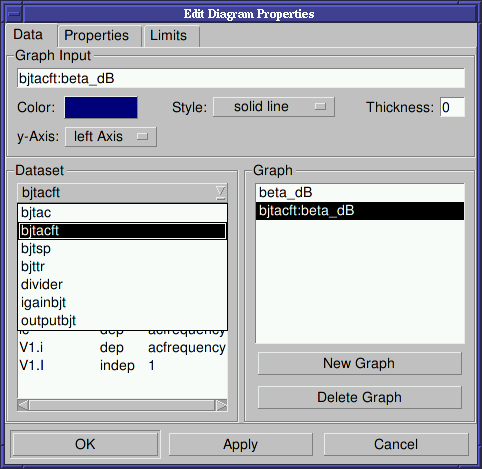
\includegraphics[width=0.7\linewidth]{diagramdialog_sets}
  \caption{Choosing graphs from different datasets}
  \label{fig:diagramdialog_sets}
\end{figure}
\FloatBarrier

The current S-parameter setup is called \textbf{bjtsp} and the setup
shown in fig.~\ref{fig:bjtacft_1} was called \textbf{bjtacft}.  Please
note that only datasets from the same project can be compared with
each other.

\tutsubsection{S-parameter and AC simulation - A Bessel band-pass filter}

The interested reader may have noticed that there seems to be a
relationship between AC analysis and the S-parameter simulation.  In
the next section we are going to explain this relationship using a
simple filter design.

\begin{figure}[ht]
  \centering
  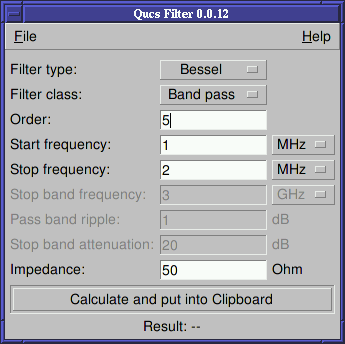
\includegraphics[width=0.55\linewidth]{besselfilter}
  \caption{Filter synthesis application}
  \label{fig:besselfilter}
\end{figure}
\FloatBarrier

In fig.~\ref{fig:besselfilter} the filter synthesis program coming
with Qucs is shown.  You can start it by the \Ctrl+\keystroke{2}
shortcut or by choosing the \textbf{Tools} $\rightarrow$
\textbf{Filter synthesis} menu entry.  The user can choose between
different types of filters and the filter class (lowpass, highpass,
bandpass or bandstop).  Also the appropriate corner frequencies and
the order must be configured.  When setup correctly you press the
\textbf{Calculate and put into Clipboard} button.  The program will
indicate if it was possible to create the appropriate filter
schematic.  If so, the application passes the schematic to the system
wide clipboard.

\medskip

Back in the schematic editor you can paste the filter design into the
schematic using the \Ctrl+\keystroke{V} shortcut or by choosing the
\textbf{Edit} $\rightarrow$ \textbf{Paste} menu entry.

\begin{figure}[ht]
  \centering
  \includegraphics[width=0.95\linewidth]{bpsp_1}
  \caption{Schematic for 5th order Bessel band-pass filter}
  \label{fig:bpsp_1}
\end{figure}
\FloatBarrier

The schematic shown in fig.~\ref{fig:bpsp_1} was automatically created
by the filter synthesis program and can be simulated as is.  It
contains the LC-ladder network forming the actual filter, the two
S-parameter ports (the AC power sources) as well the S-parameter
simulation block with the appropriate frequencies pre-configured.
Additionally there is an equation computing the transmission and
reflection of the filter network in dB.

\begin{figure}[ht]
  \centering
  \includegraphics[width=1\linewidth]{bpsp_2}
  \caption{S-parameters of the band-pass filter}
  \label{fig:bpsp_2}
\end{figure}
\FloatBarrier

The results of the S-parameter simulation are depicted in
fig.~\ref{fig:bpsp_2}.  In the logarithmic cartesian diagram the
transmission of the filter clearly shows the band-pass behaviour
between the selected frequencies 1MHz and 2MHz.  Additionally the
input- and output reflections can be seen in the two Smith charts.

\medskip

Now two AC setups will be created to calculate the same S-parameters
as found in the previous simulation.  In fig.~\ref{fig:bpac_1} the
LC-ladder network is unchanged but the S-parameter ports are replaced
by a $50\Omega$ resistor and an AC voltage source in series.  Also
there is now an AC simulation block with the same frequency sweep
chosen as in the previous S-parameter simulation.

\begin{figure}[ht]
  \centering
  \includegraphics[width=1\linewidth]{bpac_1}
  \caption{S-parameters at port 1 of the band-pass filter using AC analysis}
  \label{fig:bpac_1}
\end{figure}
\FloatBarrier

At this point some theory must be stressed.

\medskip

S-parameters are defined by ingoing (a) and outgoing (b) power waves:
\begin{align*}
a &= \dfrac{V + Z_0\cdot I}{2 \cdot \sqrt{Z_0}}\\
b &= \dfrac{V - Z_0\cdot I}{2 \cdot \sqrt{Z_0}}
\end{align*}

whereas $Z_0$ denotes the reference impedance the S-parameters will be
normalized to.  With this definition the two-port S-parameters can be
written as:
\begin{equation*}
S_{11} = \left.\dfrac{b_1}{a_1}\right|_{b_2=0}\;\;\;\;
S_{21} = \left.\dfrac{b_2}{a_1}\right|_{b_2=0}\;\;\;\;
S_{22} = \left.\dfrac{b_2}{a_2}\right|_{b_1=0}\;\;\;\;
S_{12} = \left.\dfrac{b_1}{a_2}\right|_{b_1=0}
\end{equation*}

Back at the schematic in fig.~\ref{fig:bpac_1}.  The amplitude of the
AC voltage source \textbf{V1} is set to 1V (but can be any other value
different from zero) and the side condition $\mathrm{b_2=0}$ is
fulfilled by setting the amplitude of the AC voltage source
\textbf{V2} to 0V.  The additional equations just calculate the
S-parameters as they are defined from the AC simulation values.

\medskip

Please note the current directions through the AC voltages sources
\textbf{V1.i} and \textbf{V2.i}.  They must be considered by the unary
minus in the equations.

\medskip

The results of this simulation again show the filter transmission
function as we already know it from the S-parameter simulation.  Also
the reflections at port 1 look identical.

\medskip

In the second schematic shown in fig.~\ref{fig:bpac_2} the second port
is handled.  The amplitude of the AC voltage source \textbf{V2} is set
to 1V and the side condition $\mathrm{b_1=0}$ considered by a zero AC
voltage source \textbf{V1}.  Again the appropriate equations are used
to compute the two remaining S-parameters.

\medskip

The below simulation results again verified that we can perform a
partial S-parameter analysis using the AC simulation block and some
additional equations.  The diagrams in fig.~\ref{fig:bpac_2} and
fig.~\ref{fig:bpsp_2} are identical.

\begin{figure}[ht]
  \centering
  \includegraphics[width=1\linewidth]{bpac_2}
  \caption{S-parameters at port 2 of the band-pass filter using AC analysis}
  \label{fig:bpac_2}
\end{figure}
\FloatBarrier

Recapitulating we learned from this example that a S-parameter
simulation is a number of AC simulations with some additional
calculation formulas.  This is true though the actual simulation
algorithms implemented in Qucs are completely different.
